% !TEX TS-program = pdflatex
% !TEX encoding = UTF-8 Unicode

% This file is a template using the "beamer" package to create slides for a talk or presentation
% - Giving a talk on some subject.
% - The talk is between 15min and 45min long.
% - Style is ornate.

% MODIFIED by Jonathan Kew, 2008-07-06
% The header comments and encoding in this file were modified for inclusion with TeXworks.
% The content is otherwise unchanged from the original distributed with the beamer package.

\documentclass{beamer}


% Copyright 2004 by Till Tantau <tantau@users.sourceforge.net>.
%
% In principle, this file can be redistributed and/or modified under
% the terms of the GNU Public License, version 2.
%
% However, this file is supposed to be a template to be modified
% for your own needs. For this reason, if you use this file as a
% template and not specifically distribute it as part of a another
% package/program, I grant the extra permission to freely copy and
% modify this file as you see fit and even to delete this copyright
% notice. 


\mode<presentation>
{
  \usetheme{Warsaw}
  % or ...

  \setbeamercovered{transparent}
  % or whatever (possibly just delete it)
}


\usepackage[english]{babel}
% or whatever
\usepackage{natbib}
    \renewcommand{\bibsection}{\subsubsection*{\bibname } }
\usepackage{tipa}

\usepackage[utf8]{inputenc}
% or whatever

\usepackage{times}
\usepackage[T1]{fontenc}
% Or whatever. Note that the encoding and the font should match. If T1
% does not look nice, try deleting the line with the fontenc.


\title % (optional, use only with long paper titles)
{Attention and salience in lexically-guided perceptual learning}

\author % (optional, use only with lots of authors)
{Michael McAuliffe}
% - Use the \inst{?} command only if the authors have different
%   affiliation.

% - Use the \inst command only if there are several affiliations.
% - Keep it simple, no one is interested in your street address.

\date
{530 final presentation}




% If you have a file called "university-logo-filename.xxx", where xxx
% is a graphic format that can be processed by latex or pdflatex,
% resp., then you can add a logo as follows:

% \pgfdeclareimage[height=0.5cm]{university-logo}{university-logo-filename}
% \logo{\pgfuseimage{university-logo}}



% Delete this, if you do not want the table of contents to pop up at
% the beginning of each subsection:
\AtBeginSubsection[]
{
  \begin{frame}<beamer>{Outline}
    \tableofcontents[currentsection,currentsubsection]
  \end{frame}
}


% If you wish to uncover everything in a step-wise fashion, uncomment
% the following command: 

%\beamerdefaultoverlayspecification{<+->}


\begin{document}

\begin{frame}
  \titlepage
\end{frame}

\begin{frame}{Research Questions}

\begin{itemize}
\item Listeners are constantly adapting to speech
\item How automatic is this process?
\item How context-independent or context-dependent is this process?
\end{itemize}
\end{frame}

\begin{frame}{Outline}
  \tableofcontents
  % You might wish to add the option [pausesections]
\end{frame}


% Since this a solution template for a generic talk, very little can
% be said about how it should be structured. However, the talk length
% of between 15min and 45min and the theme suggest that you stick to
% the following rules:  

% - Exactly two or three sections (other than the summary).
% - At *most* three subsections per section.
% - Talk about 30s to 2min per frame. So there should be between about
%   15 and 30 frames, all told.

\section{Background}

\begin{frame}{Definitions}
  % - A title should summarize the slide in an understandable fashion
  %   for anyone how does not follow everything on the slide itself.

    Perceptual learning
\begin{itemize}
\item Psychophysics: updating of categories to reflect actual stimuli \citep{Gibson1953}
\item Speech perception: updating sound categories in response to exposure \citep{Norris2003}
\end{itemize}
 
\end{frame}

\begin{frame}{Perceptual learning}

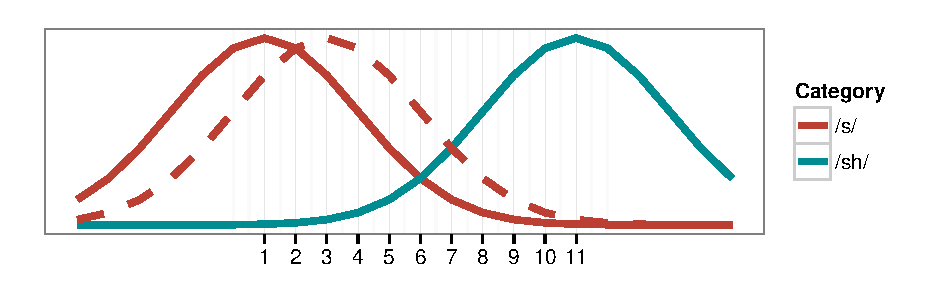
\includegraphics[width=1.1\textwidth]{graphs/dist.pdf}

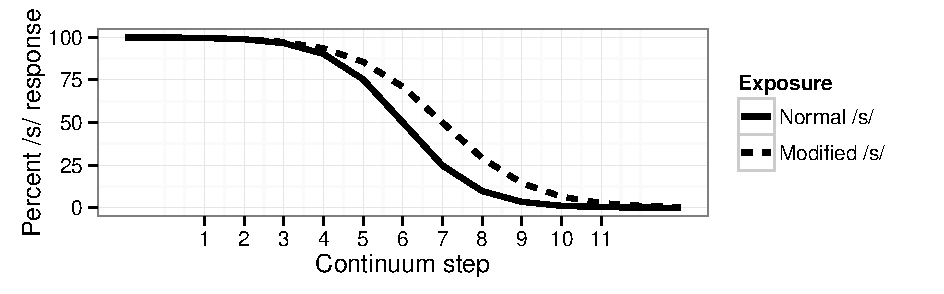
\includegraphics[width=1.1\textwidth]{graphs/class.pdf}

\end{frame}

\begin{frame}{Definitions}
  % - A title should summarize the slide in an understandable fashion
  %   for anyone how does not follow everything on the slide itself.

    Attention
\begin{itemize}
\item Selective attention to a particular sound category (/s/)
\item Feature-based attention (as opposed to singleton-based attention)
\end{itemize}
 Salience
\begin{itemize}
\item Linguistic: word-position or semantic predictability
\item Signal/linguistic: category typicality (/s/-/\textesh/)
\end{itemize}
Attentional sets
\begin{itemize}
\item Comprehension-oriented attentional set
\item Perception-oriented attentional set
\end{itemize}
\end{frame}

\begin{frame}{Theoretical framework}
\begin{columns}[T]
\begin{column}{.68\textwidth}
Predictive coding model of the brain 

\citep{Clark2013}
  \begin{itemize}
\item Hierarchical
\item Expectations propagate to lower levels
\item Error signals from unmet expectations propagate to higher levels
\item Similar computational models can account for perceptual learning \citep{Kleinschmidt2011}
  \end{itemize}
\end{column}
\hfill
\begin{column}{.3\textwidth}
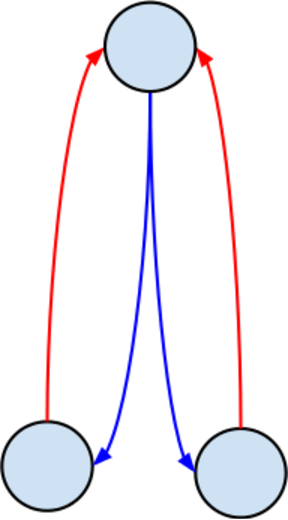
\includegraphics[width=\textwidth]{graphs/PCschema.pdf}
\end{column}
\end{columns}
\end{frame}

\begin{frame}{Attention in predictive coding}
\citet{Clark2013}
\begin{itemize}
\item Gain-based attention mechanism
\begin{itemize}
\item Attention increases weight of error signals
\item Predicts greater updating of expectations when listeners attend to the signal
\end{itemize}
\end{itemize}
This dissertation
\begin{itemize}
\item Propagation-inhibiting attention mechanism
\begin{itemize}
\item Attention resolves expectations at the attended level, inhibiting further propagation of error signals
\item Predicts that perception-oriented attentional sets will generalize less, showing smaller perceptual learning effects
\end{itemize}
\end{itemize}
\end{frame}

\section{Experiments}

\subsection{Experiment 1}

\begin{frame}{Experiment 1}
Standard lexically-guided perceptual learning paradigm
\begin{itemize}
\item Exposure
\begin{itemize}
\item Lexical decision task
\item Words with /s/ in them that sound halfway in between /s/ and /\textesh/ (~50\% /s/ response in a pretest) 
\item 2x2 design (100 participants total)
\begin{itemize}
\item Word-initial or word-medial
\item Attention to /s/ or no attention to /s/
\end{itemize}
\end{itemize}
\item Categorization
\begin{itemize}
\item Four minimal pair continua
\begin{itemize}
\item \emph{sin-shin}, \emph{sack-shack}, \emph{sock-shock}, \emph{sigh-shy} 
\end{itemize}
\item Middle six steps of each continua (as determined by a pretest) 
\item Control group completed just the categorization for comparison to experimental groups
\end{itemize}
\end{itemize}
\end{frame}

\begin{frame}{Experiment 1 results}
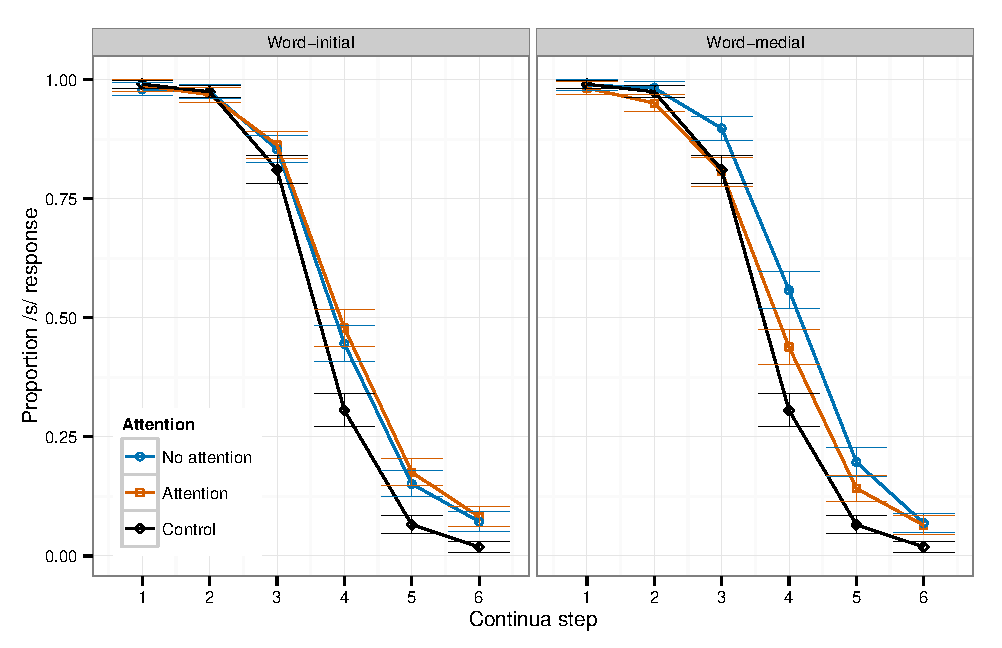
\includegraphics[width=\textwidth]{graphs/exp1_categresults_present.pdf}
\end{frame}

\subsection{Experiment 2}

\begin{frame}{Experiment 2}
Same structure as Experiment 1
\begin{itemize}
\item Exposure
\begin{itemize}
\item Lexical decision task
\item \textbf{Words with /s/ in them that sound more like /\textesh/ than /s/ (~30\% /s/ response in a pretest) }
\item 2x2 design (100 participants total)
\begin{itemize}
\item Word-initial or word-medial
\item Attention to /s/ or no attention to /s/
\end{itemize}
\end{itemize}
\item Categorization
\begin{itemize}
\item Four minimal pair continua
\begin{itemize}
\item \emph{sin-shin}, \emph{sack-shack}, \emph{sock-shock}, \emph{sigh-shy} 
\end{itemize}
\item Middle six steps of each continua (as determined by a pretest) 
\end{itemize}
\end{itemize}
\end{frame}

\begin{frame}{Experiment 2 results}
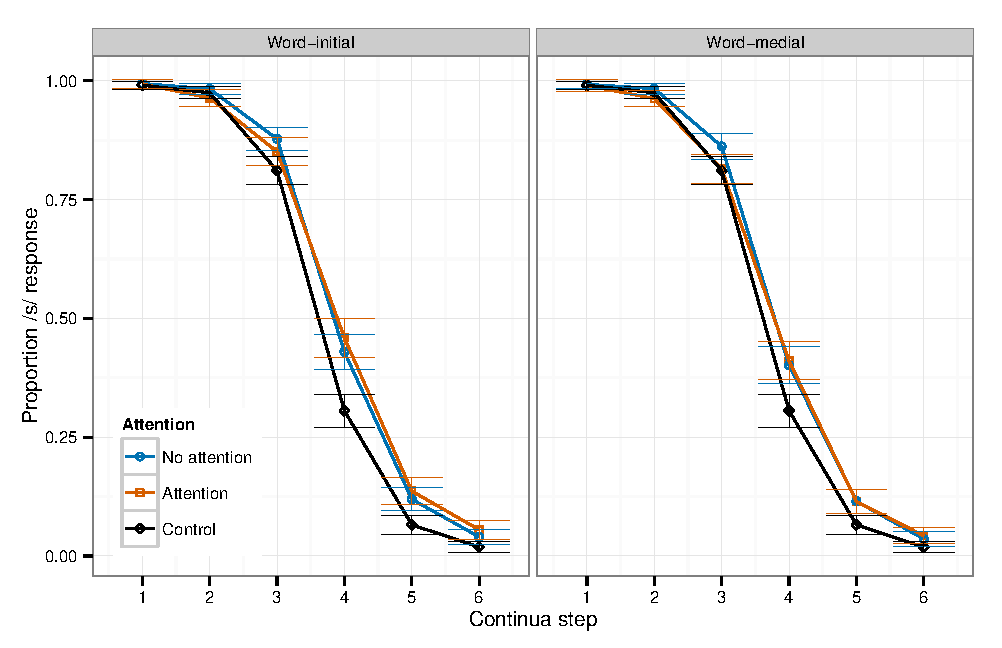
\includegraphics[width=\textwidth]{graphs/exp2_categresults_present.pdf}
\end{frame}

\begin{frame}{Influence of endorsement rate on perceptual learning}
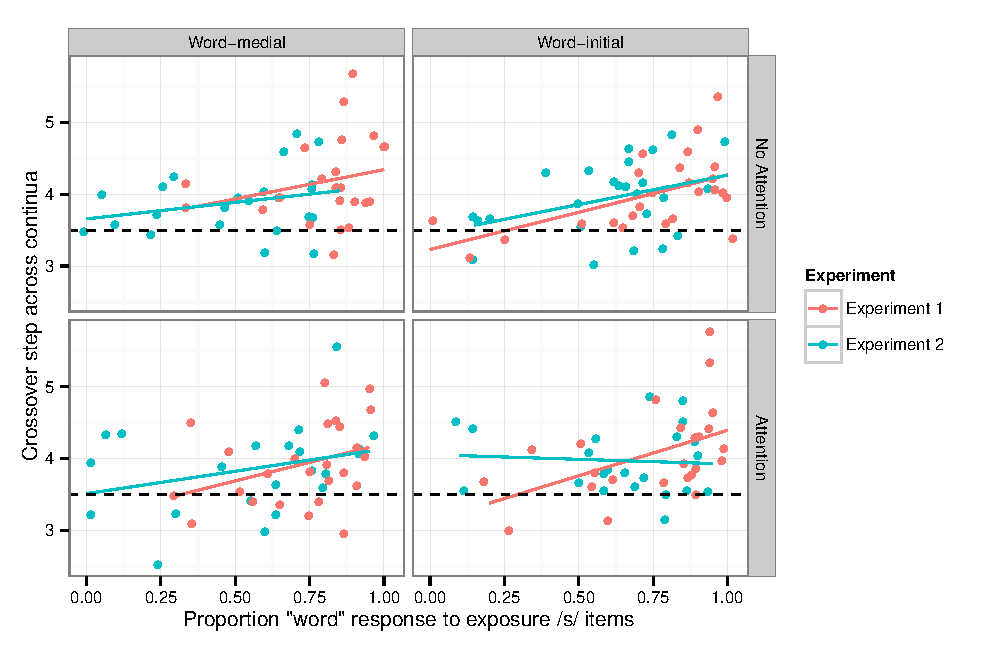
\includegraphics[width=\textwidth]{graphs/exp12_xoverwordresp_present.pdf}
\end{frame}

\subsection{Experiment 3}

\begin{frame}{Experiment 3}
Novel cross-modal word identification paradigm
\begin{itemize}
\item Exposure
\begin{itemize}
\item Auditory sentences
\item Identify the picture that corresponds to the final word in the sentence
\item Sentences can be either predictive of the final word or not
\item Words with /s/ in them that sound halfway in between /s/ and /\textesh/ (as in Experiment 1)
\item 2x2 design
\begin{itemize}
\item Words with /s/ only in predictive sentences or only in unpredictive sentences
\item Attention to /s/ or no attention to /s/
\end{itemize}
\end{itemize}
\item Categorization
\begin{itemize}
\item Identical to Experiments 1 and 2
\end{itemize}
\end{itemize}
\end{frame}

\begin{frame}{Experiment 3 results}
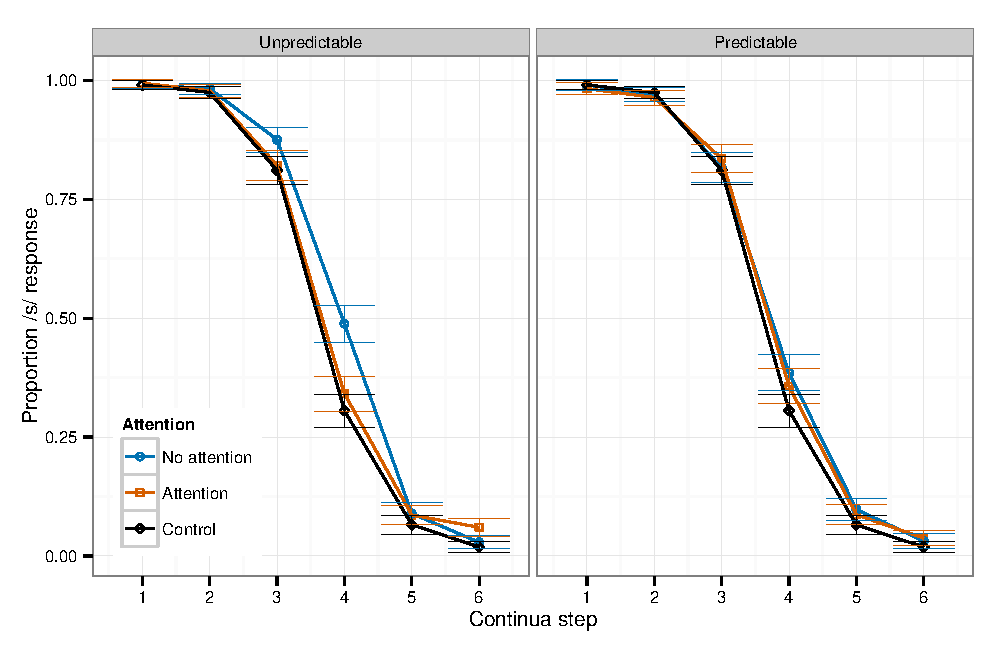
\includegraphics[width=\textwidth]{graphs/exp3_categresults_present.pdf}
\end{frame}

\section{Discussion}

\begin{frame}{Discussion}
\begin{itemize}
\item Perceptual learning effects were present for all experimental participants
\item Comprehension-oriented attentional sets
\begin{itemize}
\item Word-medial, less atypical /s/ productions produced the larger perceptual learning effects
\item Words in isolation and words in unpredictive contexts showed "larger" effects than words in predictive contexts
\end{itemize}
\item Perception-oriented attentional sets
\begin{itemize}
\item Word-initial or more atypical /s/ productions produced smaller perceptual learning effects
\item Predictive sentences are lower cognitive load, allowing for more perception-oriented attention \citep{Samuel1981}
\end{itemize}
\end{itemize}
\end{frame}

\begin{frame}{Attention switching and individual differences}
\begin{itemize}
\item Attentional sets are not fixed
\item Attention-switching control rather than selective attention and hearing loss affect perceptual learning in older adults \citep{Scharenborg2014}
\begin{itemize}
\item Listeners with worse attention-switching control show larger perceptual learning effects
\item These listeners would be oriented more towards comprehension
\end{itemize}
\item Certain individuals may be more oriented towards one attentional set or the other
\begin{itemize}
\item Global versus local processing differences
\end{itemize}
\end{itemize}
\end{frame}

\begin{frame}{Attention mechanisms}
Gain-based mechanism
\begin{itemize}
\item Cannot account for the results of these experiments
\item Increasing attention to perception always reduced perceptual learning
\end{itemize}
Propagation-inhibiting mechanism
\begin{itemize}
\item Accounts for the variability of perceptual learning effects across paradigms and fields
\begin{itemize}
\item Psychophysics perceptual learning \citep[for review]{Gilbert2001} and visually-guided perceptual learning \citep[e.g.][]{Bertelson2003} use perception-oriented tasks
\item Lexically-guided perceptual learning use comprehension-oriented tasks \citep[e.g.][]{Norris2003}
\end{itemize}
\end{itemize}
\end{frame}

\begin{frame}{Summary}

  % Keep the summary *very short*.
  \begin{itemize}
  \item
    Perceptual learning is a largely automatic process
  \item
    However, attentional sets determine the magnitude of perceptual learning effects
  \item
    These results support a propagation-inhibiting mechanism of attention in predictive coding frameworks, rather than a gain mechanism
  \end{itemize}
  
\end{frame}

\begin{frame}[allowframebreaks]%in case more than 1 slide needed
    {\footnotesize
\bibliographystyle{apalike}
\bibliography{biblio}
    }
\end{frame}


\end{document}


